\section{The model, the results and their dependencies}\label{sec:model}
\subsection{Physical filter order is retained}
The concentration-scaled original equations are
\begin{equation}\label{eq:physical}
\frac{\mathrm dx_c}{\mathrm dt_{\rm phys}}=x_c(r_0-y_c),\qquad
\frac{\mathrm dy_c}{\mathrm dt_{\rm phys}}=a_0(z_c-y_c),\qquad
\frac{\mathrm dz_c}{\mathrm dt_{\rm phys}}=b_0(x_c-z_c),
\end{equation}
where $a_0,b_0>0$ and the oscillatory regime is $r_0>a_0+b_0$.
For the usual reaction-rate convention, $r_0=\kappa_1-\kappa_4$, $a_0=\kappa_3$, $b_0=\kappa_5$, with the fixed outer-reactant concentration absorbed into $\kappa_1$. The raw concentrations are multiplied by $\kappa_2\kappa_4/a_0$, $\kappa_2$ and $\kappa_2b_0/a_0$, respectively, to obtain \eqref{eq:physical}.

Put $X=x_c/r_0$, $Y=y_c/r_0$, $Z=z_c/r_0$ and
\begin{equation}\label{eq:parameters}
t=b_0t_{\rm phys},\quad \mu=\frac{a_0}{b_0}>0,\quad
\lambda=\frac{r_0}{b_0},\quad k=\mu\lambda,\quad A=1+\mu,\quad \kH=\mu(1+\mu),\quad \rho=\frac{k}{\kH}.
\end{equation}
Primes denote this fast time $t$, unless another variable is displayed. Then
\begin{equation}\label{eq:filters}
X'=\lambda X(1-Y),\qquad Y'=\mu(Z-Y),\qquad Z'=X-Z.
\end{equation}
The intermediate filter is $Z$ and the final feedback filter is $Y$. Their order is not interchanged and $\mu\le1$ is not assumed, except where a statement says so.

The invertible change
\begin{equation}\label{eq:change}
x=kX,\qquad y=kZ,\qquad p=\lambda(1-Y),\qquad U=\log(x/k)
\end{equation}
gives
\begin{equation}\label{eq:system}
x'=px,\qquad p'=k-\mu p-y,\qquad y'=x-y,
\end{equation}
on the positively invariant domain
\[
\Dom=\{x>0,\ y>0,\ p<\lambda\},\qquad
\cP=\{(\mu,k):\mu>0,\ k>\mu(1+\mu)\}.
\]
In log coordinates,
\begin{equation}\label{eq:logsystem}
U'=p,\qquad p'=k-\mu p-y,\qquad y'=ke^U-y,
\end{equation}
and the equilibrium is $E=(0,0,k)$. Elimination gives
\begin{equation}\label{eq:scalar}
U'''+AU''+\mu U'+k(e^U-1)=0.
\end{equation}
A \emph{cycle} means the image of a nonconstant positive periodic solution with its \emph{least} period $T$, not a choice of phase or a multiple traversal. Write $\avg f=T^{-1}\int_0^T f\dd$. A solution defined for all real times is \emph{log-bounded} if $(U,p,y)$ is bounded on $\R$.

Equation \eqref{eq:scalar} is $(D+1)(D+\mu)U'=-k(e^U-1)$ with $D=\mathrm d/\mathrm dt$. Inverting the two filters on bounded solutions gives
\begin{equation}\label{eq:delay}
x'(t)=x(t)\Bigl[\lambda-\int_0^\infty G(s)\,x(t-s)\,\mathrm ds\Bigr],\qquad
G(s)=\frac{e^{-\mu s}-e^{-s}}{1-\mu}\quad(G(s)=se^{-s}\text{ if }\mu=1),
\end{equation}
the logistic equation with a two-stage distributed delay; \eqref{eq:system} is its linear-chain form \cite{Ruan06}. For a pure delay in place of $G$ this is Wright's equation, for which uniqueness of the slowly oscillating periodic solution (Jones' conjecture) was established by large-parameter asymptotics together with computer-assisted proofs \cite{Xie93,JLM17,vdBJ18,Jaquette19}.

The scalar equation \eqref{eq:scalar}, written in the time $\sqrt\mu\,t$, depends on $\mu$ only through $(1+\mu)/\sqrt\mu$, which is invariant under $\mu\mapsto1/\mu$. Cycles and their Floquet multipliers at $(\mu,\rho)$ and $(1/\mu,\rho)$ therefore correspond; the positive chemical domains do not. Corollary~\ref{cor:lgreciprocal} states the correspondence precisely.

\subsection{Main conclusions}
The question left open by Smith \cite{Smith12} and retained by Boros and Hofbauer \cite{BH23} is whether \eqref{eq:physical} has exactly one cycle for every $r_0>a_0+b_0$. This paper does not settle it for all parameters. It proves the following.

\begin{theorem}[Uniqueness at large gain, in original rates]\label{thm:mainlarge}
Let $a_0,b_0>0$ and suppose
\begin{equation}\label{eq:mainthreshold}
r_0\ \ge\ 1000\,\frac{\max(a_0,b_0)^2}{\min(a_0,b_0)} .
\end{equation}
Then \eqref{eq:physical} has exactly one positive nonconstant periodic orbit. It is hyperbolic and orbitally asymptotically stable, both transverse Floquet multipliers lie in $(0,1)$, and it attracts every positive solution that does not lie on the one-dimensional stable manifold of the positive equilibrium.
\end{theorem}
In the scaled parameters \eqref{eq:mainthreshold} reads $k\ge1000$ if $\mu\le1$ and $k\ge1000\mu^3$ if $\mu\ge1$. Theorem~\ref{thm:mainlarge} is Theorem~\ref{thm:largegain} with Corollaries~\ref{cor:lgunique} and~\ref{cor:lgreciprocal}. The constant $1000$ is not sharp, and the threshold is not uniform in $\rho$ as $\min(\mu,1/\mu)\to0$.

\begin{theorem}[The attractor is a convex planar graph]\label{thm:mainattractor}
For all $\mu,k>0$ the union $\cA$ of the log-bounded entire orbits of \eqref{eq:logsystem} is a compact connected global attractor of the flow on $\Dom$. The projection $(U,p,y)\mapsto(U,p)$ is injective on $\cA$, and $\cA$ is the graph $y=h(U,p)$ of the restriction of a convex function to the compact set $\Dsc=\pi(\cA)$; $h$ is $C^1$ in the interior of $\Dsc$. The flow on $\cA$ is conjugate to the planar flow
\[
u'=v,\qquad v'=k-\mu v-h(u,v),
\]
whose divergence in the interior of $\Dsc$ is $\eta-\mu$; here $(\zeta,-\eta)=\nabla h$ extends the adjoint ratios of Section~\ref{sec:adjoint} from cycles to all of $\cA$. If $k>\kH$, then $\Dsc$ is the closed Jordan domain bounded by the projection of the outermost cycle and $E$ is a source of the planar flow. At a parameter where every cycle satisfies $\avg\eta<\mu$, the cycle is unique; if there are at least two cycles, one of them satisfies $\avg\eta\ge\mu$.
\end{theorem}
This is Theorem~\ref{thm:attractor} and Corollary~\ref{cor:criterion}.

\begin{theorem}[Shape of every cycle and exact weak exponent]\label{thm:mainformulas}
Let $(\mu,k)\in\cP$. The projection of every cycle to the $(U,p)$ plane is a strictly convex Jordan curve, strictly star-shaped about the origin: $\Sg=p^2-Up'>0$ and $\Xg=p'^2-pp''>0$. With the convexity gauges $K,W>0$ of Section~\ref{sec:support}, the weak transverse exponent $\lambda_c=T^{-1}\log m_t$ satisfies
\begin{equation}\label{eq:mainformula}
\lambda_c=\avg\eta-\mu=-\avg{\frac{pK}{\Sg}}=-\avg{\frac{pW}{\Xg}} .
\end{equation}
Each of the three components of the weak adjoint Floquet solution has exactly two simple zeros per period, interlaced in a fixed order with the six extrema of the concentrations.
\end{theorem}
This combines Theorems~\ref{thm:gauges} and~\ref{thm:twelve}. Formula \eqref{eq:mainformula} does not determine the sign of $\lambda_c$: the integrand changes sign with $p$. Figure~\ref{fig:attractor} illustrates Theorems~\ref{thm:mainattractor} and~\ref{thm:mainformulas} at one parameter.

\begin{figure}[!htbp]
\centering
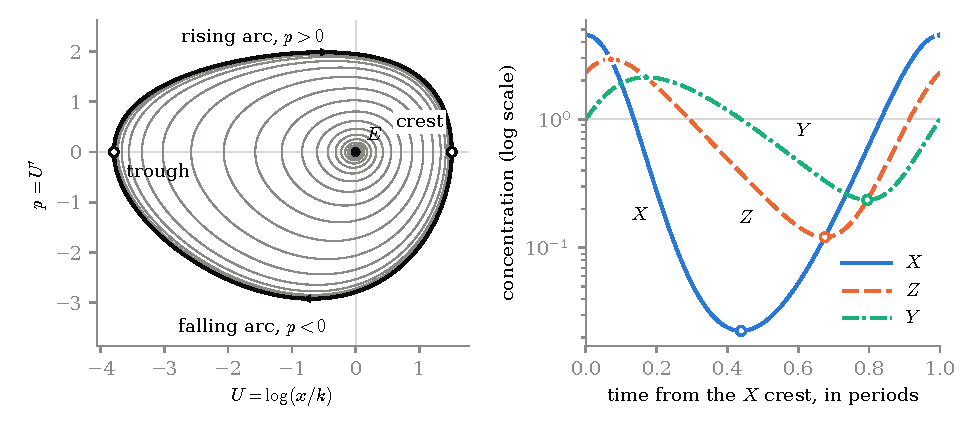
\includegraphics[width=\textwidth]{figures/fig_attractor.pdf}
\caption{Illustration at $\mu=1$, $\rho=1.3$, computed in floating point and not used in any proof. Left: projection to the $(U,p)$ plane of an orbit on the unstable manifold of $E$ (grey), which spirals clockwise out to the computed cycle (black); the projected cycle is strictly convex and star-shaped about $E$, and the rising arc ($p>0$) runs from trough to crest. Right: the three concentrations over one period on a logarithmic scale, starting at the $X$ crest; filled markers are maxima and open markers minima, in the order $X_{\max}$, $Z_{\max}$, $Y_{\max}$, $X_{\min}$, $Z_{\min}$, $Y_{\min}$ of Theorem~\ref{thm:six}.}\label{fig:attractor}
\end{figure}

\begin{theorem}[Finite-parameter obstruction, in original rates]\label{thm:main}
Fix any $a_0,b_0>0$. If \eqref{eq:physical} has more than one positive nonconstant periodic orbit at a finite growth rate $r_1>a_0+b_0$, then there is a rate
\[
a_0+b_0<r_*\le r_1
\]
at which a nonconstant positive cycle of physical least period $T_{\rm phys}$ has transverse Floquet multipliers
\begin{equation}\label{eq:physicalneutral}
1,\qquad \exp\{-(a_0+b_0)T_{\rm phys}\}.
\end{equation}
More generally, the number of cycles is constant along every compact parameter path in $\cP$ on which no cycle has an additional multiplier $+1$.
\end{theorem}
The multiplier $1$ in \eqref{eq:physicalneutral} is transverse to the autonomous tangent direction. Its existence is necessary for failure of uniqueness somewhere along the path; by itself it is not a counterexample. Theorem~\ref{thm:main} is proved in Section~\ref{sec:obstruction}.

\paragraph{What remains open.} Uniqueness is proved here in the region \eqref{eq:mainthreshold} and, by Lemma~\ref{lem:collar}, in a non-explicit right-hand neighbourhood of each Hopf point. For
\[
a_0+b_0<r_0<1000\,\frac{\max(a_0,b_0)^2}{\min(a_0,b_0)}
\]
outside those neighbourhoods the cycle count is not determined by the results of this paper. By Theorem~\ref{thm:mainattractor} the open statement is that $\avg\eta<\mu$ on every cycle; equivalent forms are collected in Section~\ref{sec:status}. Floating-point computation found no second cycle and no cycle with $\lambda_c\ge0$ (Section~\ref{sec:evidence}); that is evidence, not proof.

\subsection{A short route through the main argument}
For the principal conclusion, read the model and claim boundaries in this section,
the exact multiplier formula in Section~\ref{sec:adjoint}, the all-cycle geometric
framework in Sections~\ref{sec:support}--\ref{sec:geometry}, and the large-gain
theorem in Section~\ref{sec:largegain}. The attractor proof is in
Section~\ref{sec:attractor}; compactness and the neutral-cycle argument in
Sections~\ref{sec:compact}--\ref{sec:obstruction} explain why stability can force
uniqueness. The subsequent small-rate-ratio analysis, failed-certificate catalogue,
computational record and future programme are supplementary developments, not
additional assumptions of the large-gain theorem. The kurtosis inequality in
Theorem~\ref{thm:kurtosis} concerns general strictly convex potentials and can be
read as a reusable result independently of the oscillator application.

\subsection{Established inputs and self-contained scope}
Wilhelm and Heinrich introduced the model and analysed its local Hopf bifurcation \cite{WH95,WH96}. Smith proved that positive solutions are permanent, that the competitive Poincar\'e--Bendixson theorem applies, that above Hopf there are finitely many cycles, at least one of them orbitally asymptotically stable, and that every positive solution outside the stable manifold of the equilibrium converges to a cycle \cite[Theorems 1.1, 1.3 and 1.4]{Smith12}. Theorem 13 of Boros and Hofbauer summarises these results, includes stability through the critical value, and retains the cycle-count question \cite{BH23}. The mass-conserving extension in that paper is a different equation.

The sections below state at each use which of these inputs is required. Section~\ref{sec:attractor} proves dissipativity and the structure of the attractor directly and uses only classical planar and invariant-manifold theory. The remaining imported tools are Perron--Frobenius theory for a strictly positive evolution, smooth dependence of solutions on data, the implicit-function theorem, the Jordan curve theorem, the planar Poincar\'e--Bendixson theorem, local Hopf theory, and, for Theorem~\ref{thm:wedge} only, Eldering's invariant-graph persistence theorem \cite{Eldering13}. Appendix~\ref{app:hopf} reproduces the Hopf coefficient in a specified convention.

The full 1995 and 1996 articles of Wilhelm and Heinrich were not obtained; their publisher records and later primary accounts were inspected. No model-specific theorem is imported from a text that was not read. The classical results are listed with references at the point of use (Sections~\ref{sec:attractor} and~\ref{sec:wedge}) and are quoted in their standard form; their original sources were not re-read for this paper. For the revised local wedge result, Theorem~3.2 and Remark~3.3 of \cite{Eldering13} and the author's errata were inspected directly; Lemma~\ref{wed:lem:slowgraph} verifies their application. The Fenichel and Jones originals remain an access gap, but are not load-bearing for this revision.

\subsection{Positioning}
The literature search behind this subsection was bounded (citation graphs of \cite{Smith12,BH23,WH95,WH96}, preprint servers and keyword searches to 3 October 2026). It found no result that resolves or partially resolves the cycle count, and no published uniqueness theorem whose hypotheses the system satisfies. A bounded negative search does not establish priority. Table~\ref{tab:positioning} separates what is taken from the literature, what is a direct proof of a phenomenon known in a general theory, and what is advanced as new.

{\small
\begin{longtable}{p{0.36\textwidth}p{0.17\textwidth}p{0.39\textwidth}}
\caption{Positioning of the results. ``New'' means: not found in the sources inspected; priority is not otherwise established.}\label{tab:positioning}\\
\toprule
Result & Status & Relation to the literature\\
\midrule
\endfirsthead
\toprule
Result & Status & Relation to the literature\\
\midrule
\endhead
\bottomrule
\endfoot
Permanence; convergence to a cycle off the stable manifold of $E$; finitely many cycles, one stable; critical global stability & imported & \cite{Smith12}, \cite[Theorem 13]{BH23}\\
Supercritical Hopf bifurcation & imported, recomputed & \cite{WH96}; Appendix~\ref{app:hopf}\\
Linear-chain form of the distributed-delay logistic equation & known & \cite{Ruan06}; only local Hopf results are available for the strong kernel\\
\midrule
Real positive transverse multipliers (Proposition~\ref{prop:multipliers}) & direct proof & general competitive and cyclic feedback theory \cite{MPS90}\\
Injective planar projection of a cycle; one crest; order of extrema (Theorems~\ref{thm:geometry}, \ref{thm:six}) & direct proof & limit sets of competitive systems project injectively \cite{Hirsch82}; monotone cyclic feedback \cite{MPS90}\\
The attractor is a two-dimensional graph bounded by a cycle (part of Theorem~\ref{thm:attractor}) & direct proof for this model & analogues for scalar delay equations \cite{Walther95}; these allow several nested cycles\\
\midrule
Strict supporting planes between bounded orbits (Theorems~\ref{thm:support}, \ref{thm:twoorbit}) & new & mechanism related to convex carrying simplices \cite{Baigent13}\\
Convexity and $C^1$ regularity of the attractor graph; planar divergence $\eta-\mu$; parameter-wise criterion (Theorem~\ref{thm:attractor}, Corollary~\ref{cor:criterion}) & new & ---\\
Convex star-shaped projections; exact formulas \eqref{eq:mainformula}; scalar Riccati reduction (Theorem~\ref{thm:gauges}, Proposition~\ref{prop:kappa}) & new & the gauges are the angular and curvature functions used in planar Dulac criteria \cite{GG21}, whose hypotheses fail here\\
Weak-adjoint zero order; strong-stable supporting planes (Theorems~\ref{thm:twelve}, \ref{thm:dualsupport}) & new & uses the sign structure of \cite{MPS90}\\
Uniform compactness of cycle families; neutral-cycle obstruction (Theorems~\ref{thm:compact}, \ref{thm:neutral}) & new & ---\\
Uniqueness for large gain with an explicit threshold (Theorem~\ref{thm:largegain}) & new & large-parameter step of the proof of Jones' conjecture \cite{Xie93} is the analogue\\
Kurtosis bound for convex potentials; local wedge theorem (Theorems~\ref{thm:kurtosis}, \ref{thm:wedge}) & proposed new results & slow-graph property derived in Lemma~\ref{wed:lem:slowgraph} using \cite{Eldering13}\\
Failure of specific certificates (Section~\ref{sec:negative}) & new negative results & hypotheses of \cite{Massera54,Zhang86,SmithHL86,SV10,GG21} tested and found to fail\\
\end{longtable}}

\paragraph{Comparison with convex carrying simplices.}
Baigent's discrete-time criterion \cite[Section~4, Theorem~6.1]{Baigent19}
assumes a face-preserving competitive Kolmogorov diffeomorphism and controlled
images of planes. Mierczy\'nski \cite[Sections~2--3]{Mierczynski20} obtains
regularity from convexity for carrying simplices under hypotheses including
forward and backward invariance of coordinate faces. Those hypotheses do not
hold for the Wilhelm--Heinrich flow in its physical coordinates: at $y=0,z>0$
the derivative $y'=a_0z$ points into the interior, and at $z=0,x>0$ one has
$z'=b_0x>0$. Thus these theorems do not directly supply the present graph result.
The specific contributions here are the strict supporting inequality between
bounded entire trajectories, its positive-adjoint supporting planes, the graph
in logarithmic coordinates, and the reduced divergence formula. This comparison
is not a claim that a different transformation or another theorem cannot apply.
In particular, the full text of Li's 1981 third-order uniqueness work was not
obtained, so its applicability and any resulting priority implications remain
unresolved. Here ``convex graph'' always means a graph of a convex function,
not a convex subset of $\R^3$.

\subsection{Notation}
Table~\ref{tab:notation} lists the symbols used throughout. Sections that need further symbols introduce them in their first paragraph.

{\small
\begin{longtable}{p{0.42\textwidth}p{0.52\textwidth}}
\caption{Global notation.}\label{tab:notation}\\
\toprule
Symbol & Meaning\\
\midrule
\endfirsthead
\toprule
Symbol & Meaning\\
\midrule
\endhead
\bottomrule
\endfoot
$\mu,\ k,\ A,\ \lambda,\ \kH,\ \rho$ & parameters \eqref{eq:parameters}; $\delta=k-\kH$; $\cP$ the oscillatory domain\\
$t$, $\tau=\sqrt\mu\,t$ & fast time; frequency-one time\\
$(U,p,y)$, $x=ke^U$, $E$ & state \eqref{eq:logsystem}; equilibrium $(0,0,k)$\\
$X,Y,Z$; $\ell=\lambda-p$ & chemical variables \eqref{eq:filters}; $\ell=\lambda Y>0$\\
$T$, $\avg{\cdot}$ & least period of a cycle; time average over it\\
$\eta,\zeta$; $\gamma=1+\avg\eta$ & positive adjoint ratios \eqref{eq:ratios}; principal adjoint exponent\\
$m_s<m_t$; $\lambda_c=\avg\eta-\mu$ & transverse Floquet multipliers; weak exponent\\
$\gamma_E,\eta_E,\zeta_E$ & adjoint data of the equilibrium (Corollary~\ref{cor:cones})\\
$K,\ W,\ \LamE$ & convexity gauges \eqref{eq:positiveK}, \eqref{eq:curvature}, \eqref{eq:LambdaE}\\
$\psiU(U)=Ue^U-e^U+1$, $\Rem(d)=e^d-1-d$ & convex remainders\\
$\Sg=p^2-Up'$, $\Xg=p'^2-pp''$ & star gauge; convexity gauge of the projected cycle\\
$\kappa=K/\Sg$; $\etaz$ & gauge ratio; explicit state function with mean $\mu$ (Theorem~\ref{thm:gauges})\\
$M$; $M_{(U,z)}$ & crest-return derivative in $(U,y)$; in $(U,z)$, $z=y/k$\\
$C$; $C_\pm$ & compound matrix \eqref{eq:compound}; cones \eqref{eq:cones}\\
$e_s=(a,-b,-c)$; $\mathfrak r=b/a$, $\mathfrak s=c/a$; $\Psi$ & strong-stable Floquet vector and ratios; weak adjoint\\
$\cA$, $\Dom$, $\pi$, $\Dsc$, $h$ & attractor, chemical domain, projection to $(U,p)$, $\pi(\cA)$, graph function\\
$D$; $\Dt$ & $\mathrm d/\mathrm dt$ in operator identities; derivative of a state function along the flow\\
\end{longtable}}
